%% ==============================
\chapter{\iflanguage{ngerman}{Design}{Concept}}
\label{sec:concept}
%% ==============================


\todo{Formulierung}
Nachdem im vorherigen Kapitel die Methode der Implementierung vorgestellt wurde, beschäftigt sich dieses mit dem Softwaredesign der Implementierung dieser.
\newline
Die Implementierung dieser Bachelorarbeit teilt sich dabei in zwei verschieden Programme auf. Zum einen den sogenannten \textit{VolumeRenderHelper}, der für das Laden, Umwandeln, Verarbeiten und Speichern der Volumendaten zuständig ist. Zum anderen das Unityprogramm \textit{VolumeRenderer}, welches zur Visualisierung der vom Helper erzeugten Daten dient. Diese beiden Programme existierten bereits vor dieser Arbeit und sind in Vorarbeiten des IPRs entstanden. In dieser Bachelorarbeit wurde der \textit{VolumeRenderHelper} um die vorgestellte Transferfunktion erweitert und der \textit{VolumeRenderer} geringfügig angepasst. Die Beiden Programme werden im folgenden als Helper und Renderer erwähnt. Weiterhin wurde ein Pythonskript \textit{PlotHelper} geschrieben, um LH-Histogramme anzuzeigen.
\newline
\todo{christians paper}
\todo{unity und stefffens zeug genauer erklären}
\todo{csharp erwähnen und allgemeine umgebung}
Anfangs liegen die CT-Daten von den Volumen in mehreren Dateien als Schnittbilder im DICOM Format vor. Diese werden mithilfe der MITK Workbench zu einer einzelnen Datei im .nrrd Format umgewandelt, da nur Volumen in diesem Format vom Helper eingelesen werden können.
\newline
Die interne Speicherung des Volumens wird mit der generischen Klasse \textit{Volume} umgesetzt. Diese besitzt ein dreidimensionalen Array vom angegebenen generischen Datentyp, sowie Informationen über das Volumen, wie zum Beispiel Größe der Voxel oder Anzahl der Elemente pro Achse. Des Weiteren bietet die Klasse verschieden Funktionen um Informationen auszulesen oder zu bearbeiten. Zur Darstellung von dreidimensionale Koordinaten, werden die Klassen \textit{IVector3} und \textit{FVector3} benutzt. Diese stellen Vektoren dar, die entweder Integer, Ganzzahlen, oder Float, Dezimalzahlen, als $x,y$ und $z$ Werte speichern.
\todo{attribute funktionen etc. von volumenklasse in UML}
\newline
\todo{mergecluster oder clustermerge}
Die Interaktion des Benutzers mit dem Helper findet über eine Kommandozeile statt. Hierbei hat der Anwender die Befehle Load, Dump, Resample, Info, Write, LHHistogram, ClusterVolume und MergeCluster zur Auswahl. Jedes Modul hat dabei seine eigene Syntax die mithilfe eines Help Befehls angezeigt werden kann.
\newline
Die Funktionen der Module entsprechen deren Namen. So lädt Load bespielsweise eine .nrrd oder binäre Datei, Dump und Write speichern das geladene Volumen als binäre oder .nrrd Datei ab, Info gibt Informationen über das aktuell geladene Volumen zurück und Resample lässt den Anwender die Größe des Volumens verändern. Ruft man den Dump Befehl mit einem $u$ am Ende auf, so wird das Volumen vor dem Speichern zum Typ $unsigned$ $int$ gecastet. Dies geschieht indem auf alle Werte der Betrag des minimalen Wertes aufaddiert wird. Dadurch verschieben sich die Werte so, dass das Minimum bei null liegt, also nur noch positive Zahlen im Volumen vorhanden sind. Dies ist für die Darstellung im Renderer wichtig, da dieser nur mit positiven Zahlen funktioniert.
\newline
Im Folgenden werden hauptsächlich die Module LHHistogram, ClusterVolume und MergeCluster erläutert, da diese im Laufe dieser Arbeit entstanden sind. LHHistogram berechnet das LH-Histogramm des geladenen Volumens und speichert dieses in einer .csv Datei ab. ClusterVolume kalkuliert ebenfalls die LH-Werte des Volumens, führt jedoch hinterher noch die beiden Clusteringsschritte des Verfahrens aus. Als Ausgabe speichert das Modul eine binäre Datei eines Volumens, in welchem die verschiedenen IDs der Cluster gespeichert sind. Die Idee dahinter wird im laufe diese Kapitels erklärt. Das Modul MergeCluster dient der Verschmelzung der gewünschten IDs mit dem ursprünglichen Volumen. Das Ergebnis dessen, ist eine finale binäre Datei, die im Renderer das Ventrikelsystem visualisiert. Ein Überblick über den gesamten Aufbau und Ablauf der Implementierung ist in  \autoref{fig:ueberblick} zu sehen.

\begin{figure}
\centering 
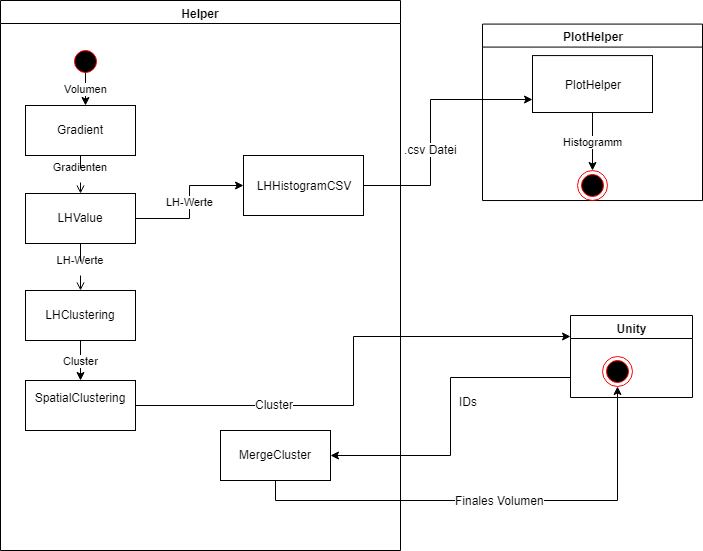
\includegraphics[width=\textwidth]{Logos/Ueberblick.png}
\caption{Überblick über das Programm} 
\label{fig:ueberblick} 
\end{figure}


Damit das Verfahren funktioniert, muss das geladene Volumen als "unsigned int" vorliegen. Der Ablauf der Berechnung startet in der statischen \textit{Gradient} Klasse. Diese ist eine Implementierung des Verfahren von Hong \cite{hong2003method}. Sie nimmt für ihre Berechnung als Parameter ein Volumen von Integern entgegen und gibt ein Volumen mit dem generischen Datentyp \textit{FVector3} zurück. Diese ist eine Hilfsklasse zur Darstellung von dreidimensionalen Vektoren.

Als nächstes wird die Funktion \textit{LHValueVolume} der statischen Klasse \textit{LHValues} aufgerufen. Diese berechnet für das gegebene \textit{FVector3} Volumen und den dazugehörigen Intensitätswerten die LH-Werte für jeden Voxel. Diese gibt die Methode in Form eines Volumens vom Typen "Tuple<float,float>" zurück.

Hat der Benutzer das Modul LHHistogram aufgerufen, entsteht im Anschluss das LH-Histogramm in der Klasse \textit{LHHistogramCSV} und wird von ihr als .csv Datei in einem vom Anwender angegebenen Pfad abgespeichert. Diese kann der Benutzer anschließend in dem Pythonscript \textit{PlotHelper}  laden und sich Visualisieren lassen. Hierbei ist zu beachten, dass das Histogramm gebildet wird, indem die Häufigkeit des Vorkommens eines LH-Wertpaares im Volumen im jeweils dazu passenden Kästchen gespeichert wird. Dies ist simpler als das im Paper von Nguyen \cite{nguyen2012clustering} benutzte Erstellen des Histogramms abhängig von einer für jeden Voxel berechneten Gewichtung. Da die Arbeit an der Implementierung zeitlich beschränkt war, wurde diese Gewichtung, die einzig und allein einer genaueren Darstellung des für das Verfahren irrelevante LH-Histogramm dient, vernachlässigt. Die Gewichtung ist für das Clustering belanglos, da dort ein Histogramm wie oben beschrieben, abhängig von der Häufigkeit der LH-Werte verwendet wird. 


Wurde jedoch das ClusterVolume Modul aufgerufen, wird mit den beiden Clusteringschritten fortgefahren.
Die Berechnung die in der \textit{LHClustering} Klasse geschieht nimmt das Volumen mit den LH-Werten entgegen und rechnet es aus Performancegründen in ein ein Histogramm um. Dieser Schritt könnte gespart werden, wenn die Methode \textit{LHValueVolume} direkt ein Histogramm als Rückgabewert liefern würde. Als Ergebnis der Clusteringfunktion \textit{ComputeLHClusters} wird eine Liste der Cluster zurückgegeben. Ein Cluster besteht aus einer Liste von \textit{IVector3}.Diese Hilfsklasse beschreibt wie \textit{FVector3} Vektoren, jedoch können die Werte nur ganze Zahlen annehmen, folglich eigenen sie sich gut, wie hier verwendet, zum Beschreiben von Positionen im Volumen.Die Cluster werden nur als Liste der räumliche Information der Punkte gespeichert, da für den nächsten Clusteringschritt  lediglich diese Information benötigt wird. 



Dies wird für jeden Voxel im Volumen berechnet. Als Ergebnis des Verfahrens kommt ein Volumen, in dem alle Gradienten gespeichert sind, heraus. Jedoch sind die Punkte um eine halbe Voxellänge verschoben. Desweiteren ist die Dimension dieses Volumens in jeder Achse um eins kleiner als das vorher gegebene Intensitätsvolumen.
Da für die Berechnung der LH-Werte jedoch der Gradient und der Intensitätswert an einer Stelle im Volumen bekannt sein muss, wurden die Intensitätswerte auf das Volumen der Gradienten umgerechnet. Dies geschieht durch eine einfach Interpolation, indem von allen 8 Nachbarn eines Punktes der Intensitätswerte aufaddiert und hinterher durch acht geteilt werden. Hierbei gehen Information verloren....
\todo{abbildung für interpolation und beschreiben was verloren geht}




Nachdem alle Cluster erzeugt wurden, werden ihnen zufällige IDs von eins bis zur Anzahl an Clustern zugeteilt. Anschließend wird ein Volumen erstellt, mit den Dimensionen des ursprünglichen Intensitätsvolumens, dass nur mit nullen als Werte gefüllt ist. Warum es diese Dimension haben muss, wird später erklärt. Danach wird durch alle Cluster iteriert, und jeder Voxel in das neu erstellte Volumen an der jeweiligen Position eingetragen. Dabei ist der eingetragene Wert immer die  ID des aktuellen Clusters. Nachdem alle Cluster abgearbeitet wurden, besteht das Volumen aus ausschließlich nullen und den IDs der Cluster an den passenden Stellen.
\newline
Dieses Volumen wird als eine binäre Datei abgespeichert und in Unity geladen. Hier kann der Anwender sich entweder die Form von einzelnen IDs anschauen oder eine Reichweite von IDs. Die gewählten IDs werden rot markiert und sich deutlich vom restlichen Volumen zu unterscheiden. Mithilfe der Darstellung muss der Nutzer anhand der Form die Cluster erkennen, die zum Ventrikelsystem gehören, und deren IDs notieren. 
\newline
Hat er dies getan kann er im ... Programm die binäre Datei mit den IDs, die ursprüngliche Intensitätsvolumendatei laden und eine die Liste der passenden IDs als Parameter übergeben. Die ausgewählten IDs werden zu einem Cluster verschmolzen und in das Intensitätsvolumen übernommen. Dort erhalten sie, da der maximale Wert von CT-Daten bei ...(4400) liegt, den Wert 5000. Dieser Wert erhöht das Maximum für die Darstellung der Daten nur gering, ist dafür aber im Volumen sonst nirgends enthalten. Das Ergebnis dieser Verschmelzung wird wieder als binäre Datei gespeichert.
\newline
Als letzten Schritt kann nun der Benutzer die verschmolzene Datei erneut in Unity laden. Hier kann er sich dann das Volumen normale abhängig von den Grauwerten dargestellt anzeigen lassen, mit dem Ventrikelsystem in rot, oder einer anderen ausgewählten Farbe darin.
\todo{letzten schritt genauer}